\documentclass{article}

\usepackage[english]{babel}
\setlength\parindent{0pt} % Removes all indentation from paragraphs
%\usepackage{times} % Uncomment to use the Times New Roman font

\usepackage{color}
	\definecolor{darkred}{rgb}{0.55, 0.0, 0.0}
	\definecolor{keywords}{RGB}{255,0,90}
	\definecolor{comments}{RGB}{0,0,113}
	\definecolor{red}{RGB}{160,0,0}
	\definecolor{green}{RGB}{0,150,0}

\usepackage{amssymb,amsmath}
\usepackage{mathtools}

\usepackage{placeins}

\usepackage{wrapfig}
\usepackage{graphicx}
\usepackage{caption}
\usepackage{subcaption}

\usepackage{hyperref}

\usepackage{listings}
\lstset{language=Python, 
        basicstyle=\ttfamily\small, 
        keywordstyle=\color{keywords},
        commentstyle=\color{comments},
        stringstyle=\color{red},
        showstringspaces=false,
        identifierstyle=\color{green},
        title=\lstname}
%------------------------------------------------------------------------------%
%------------------------------------------------------------------------------%                                   
\title{Machine Learning \\ \bf{Exercise 2: Linear/Quadratic Discriminant Analysis} } % Title
%------------------------------------------------------------------------------%                                   
% Document
%------------------------------------------------------------------------------%                                   

\begin{document}

\maketitle

\begin{center}
\begin{tabular}{l l}
Group: &  Sergej Kraft \\
       & Elias Roeger \\
       & Ekaterina Tikhoncheva \\ 
\end{tabular}
\end{center}

\tableofcontents

\section{Data Preparation}

In this exercise we use the digit data set from {\it http://scikit-learn.org/stable/datasets/}.
The main task is to write a classifier that should distinguish digit '1' from digit '7'. 

\begin{figure}
        \centering
        \begin{subfigure}[b]{0.5\textwidth}
                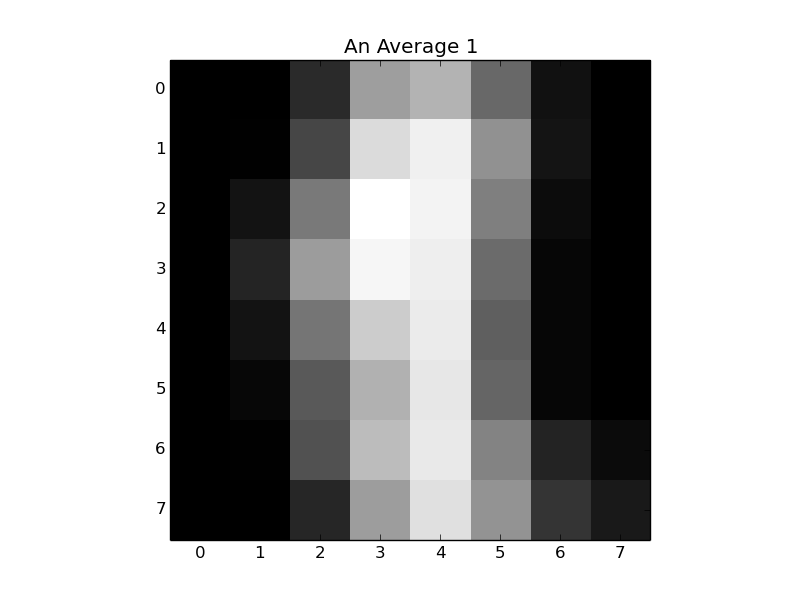
\includegraphics[width=\textwidth]{../average1.png}
                \caption{An average '1'}
        \end{subfigure}%
        \begin{subfigure}[b]{0.5\textwidth}
                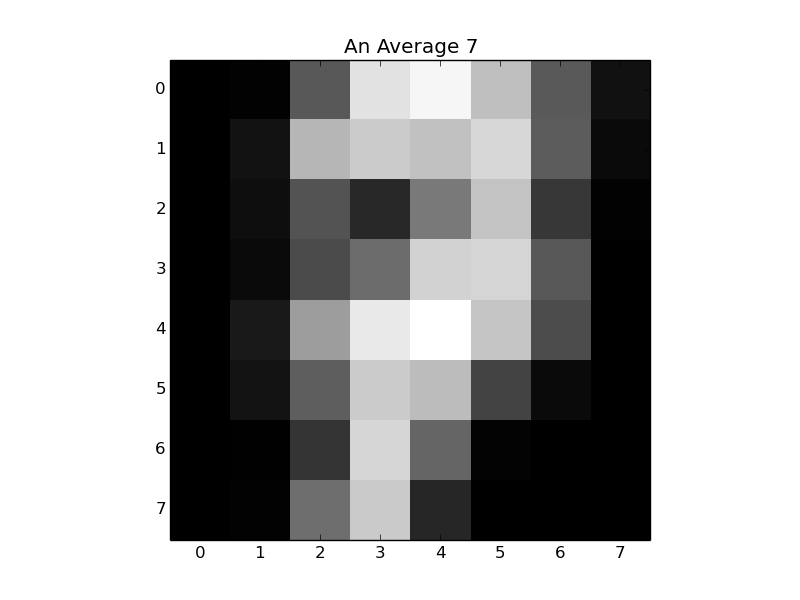
\includegraphics[width=\textwidth]{../average7.png}
                \caption{An average '7'}
        \end{subfigure}
        \caption{Average digits inside each class}\label{img1}
\end{figure}

The initial set of '1' and '7' consist of 361 Images, where each image is represented as a vector in $64$-dimensional space. For purposes of this exercise we restrict ourself to $2$-dimensional feature space. To do this we compute an average digit inside of each class (see image \ref{img1}) and then the difference between this two average digits. We select two dimensions where the calculated difference has two biggest values.

To decide if the selected features are suitable for classification we draw a distribution of data points in the feature space (see image \ref{img2}).

\begin{figure}[ht]
	\centering
  	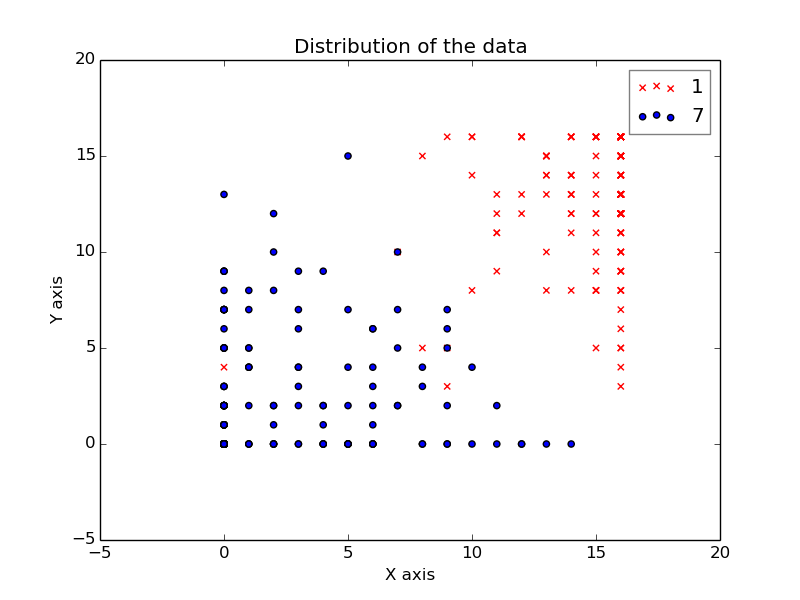
\includegraphics[width=0.7\textwidth]{../dataDistribution.png}
	\caption{Distribution of the data points in the feature space}
	\label{img2}
\end{figure}

We can see that the points of the different classes excluding several points are good separated.

For realisation of dimension reduction see function $dr(x,y)$, where $x$ is the initial set of data points and $y$ is an array of corresponding labels. The function $scatterplot(x,y,labels, title, imageName)$ implements the drawing of a scatter plot of the points.

\FloatBarrier

\section{Nearest Mean Classifier}

Implementation of the Nearest Mean Classifier

\lstinputlisting[language=Python]{NearestMean.py}

Our implementation of the Nearest Mean Classifier provides the classification rate $99.31\%$. 

\section{Quadratic Discriminant Analysis (QDA)}

Our implementation of the QDA - Training to compute the mean vectors, covariance matrices and priors of the classes.

\lstinputlisting[language=Python]{QDAtraining.py}

Our implementation of the QDA - Prediction :

\lstinputlisting[language=Python]{QDAprediction.py}

The run test on the training and test sets are present in the Table \ref{Table1}, the decision boundary of QDA is visualised on the image \ref{img3}. We also visualised the results of the classification. The correct classified points are marked with bigger symbols (see image \ref{img4}).

We can see that the QDA has a higher classification rate. The misclassifications stem from the not perfect distribution of the set points in the feature space : some point of one class lie between the points of the other class and thus on the wrong side of the decision boundary.

\begin{table}[htb]
	\centering
	\begin{tabular}{|l | c|}
		\hline
		Set & Correct Classification rate \\ \hline
		training set & $97.22\%$  \\ 
		test set &  $99.31\%$ \\ \hline 
	\end{tabular}
\caption{Correct Classification Rate of QDA}
\label{Table1}
\end{table}

\begin{figure}[ht]
	\centering
  	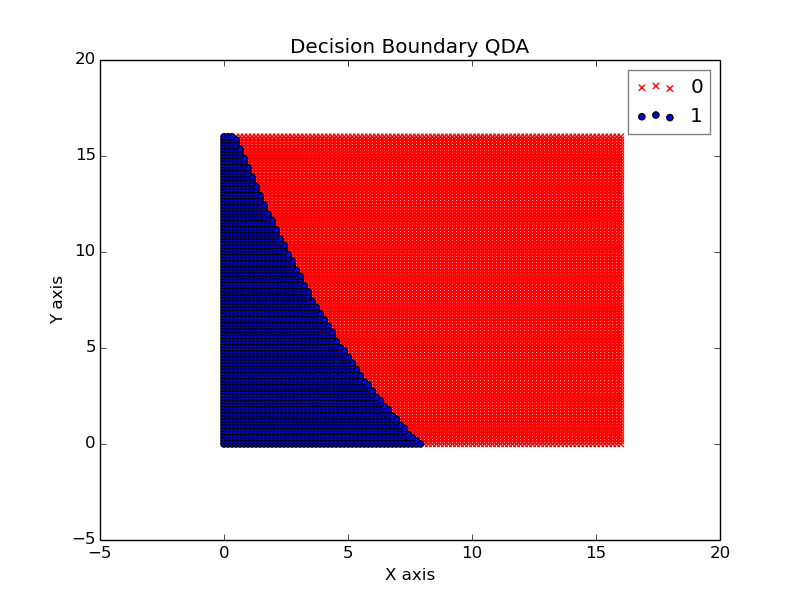
\includegraphics[width=0.7\textwidth]{../DecisionBoundaryQDA.png}
  	\caption{Decision boundary of the QDA}
	\label{img3}
\end{figure}


\begin{figure}
        \centering
        \begin{subfigure}[b]{0.5\textwidth}
                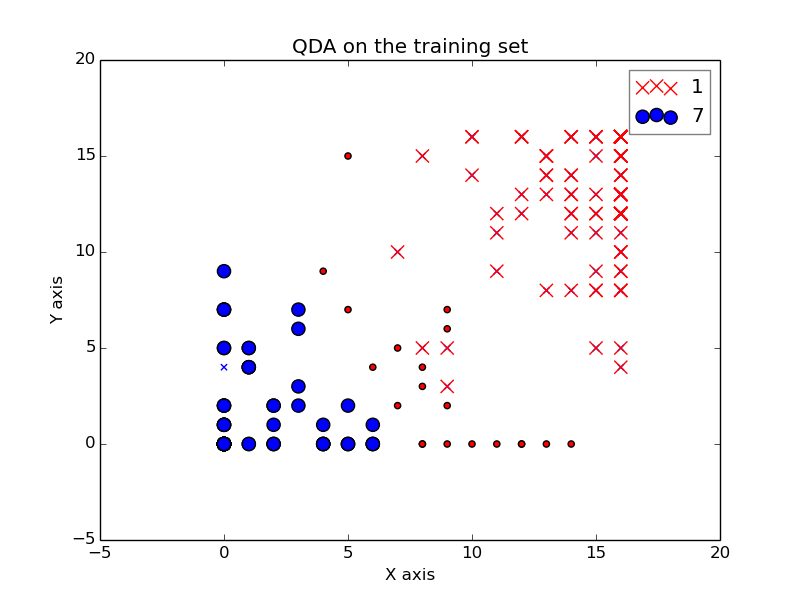
\includegraphics[width=\textwidth]{../QDAtrainingset.png}
                \caption{Training set}
        \end{subfigure}%
        \begin{subfigure}[b]{0.5\textwidth}
                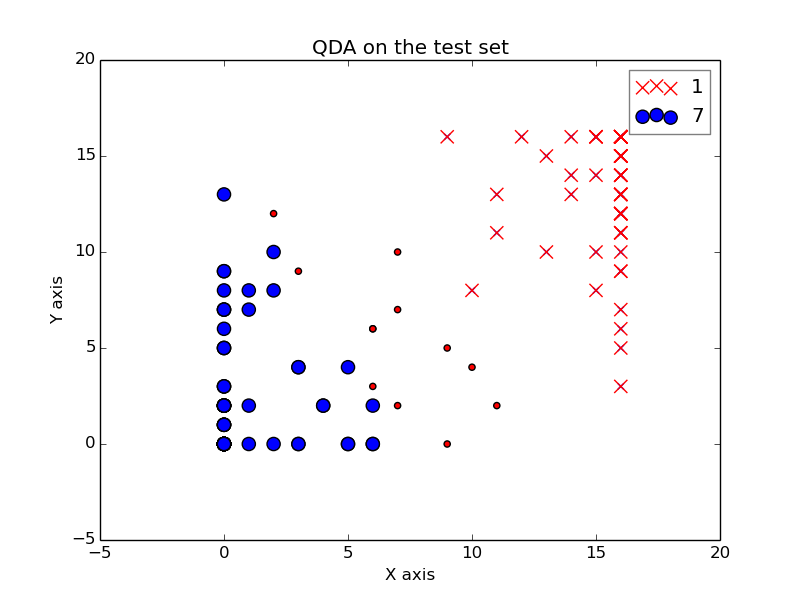
\includegraphics[width=\textwidth]{../QDAtestset.png}
                \caption{Test set}
        \end{subfigure}
        \caption{Results of QDA Prediction}
        \label{img4}
\end{figure}


\FloatBarrier

\section{Linear Discriminant Analysis (LDA)}

Implementation of the LDA prediction: 

\lstinputlisting[language=Python]{LDAprediction.py}

The run test on the training and test sets are present in the Table \ref{Table2}, the decision boundary of LDA is visualised on the image \ref{img5}. The results of the classification are presented on the image \ref{img6}.

One can see, that LDA provides lower classification rate as QDA.
\begin{table}[htb]
	\centering
	\begin{tabular}{|l | c|}
		\hline
		Set & Correct Classification rate \\ \hline
		training set & $93.06\%$  \\ 
		test set &  $95.86\%$ \\ \hline 
	\end{tabular}
\caption{Correct Classification Rate of LDA}
\label{Table2}
\end{table}

\begin{figure}[ht]
	\centering
  	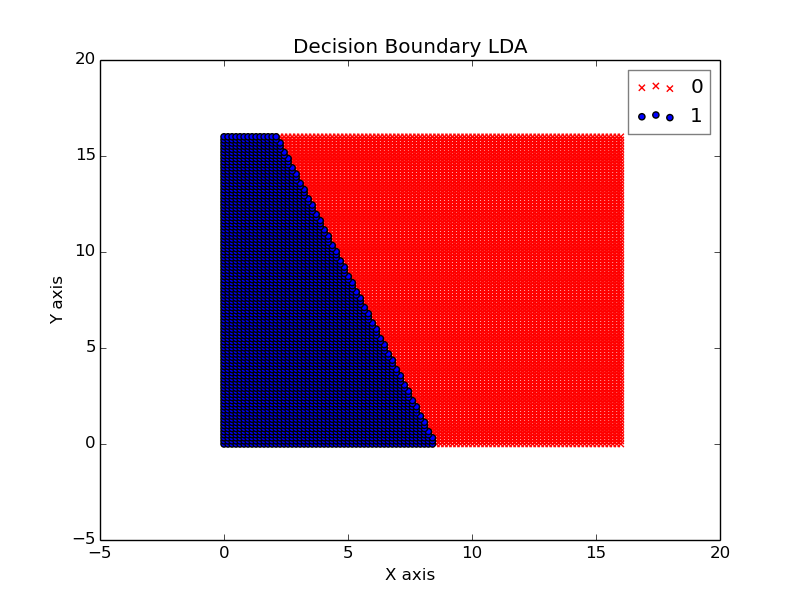
\includegraphics[width=0.7\textwidth]{../DecisionBoundaryLDA.png}
  	\caption{Decision boundary of the LDA}
	\label{img5}
\end{figure}


\begin{figure}
        \centering
        \begin{subfigure}[b]{0.5\textwidth}
                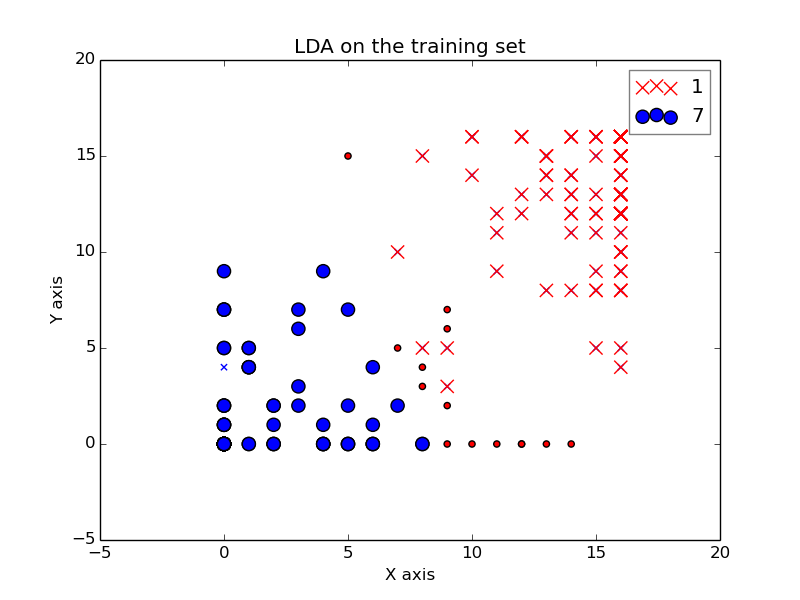
\includegraphics[width=\textwidth]{../LDAtrainingset.png}
                \caption{Training set}
        \end{subfigure}%
        \begin{subfigure}[b]{0.5\textwidth}
                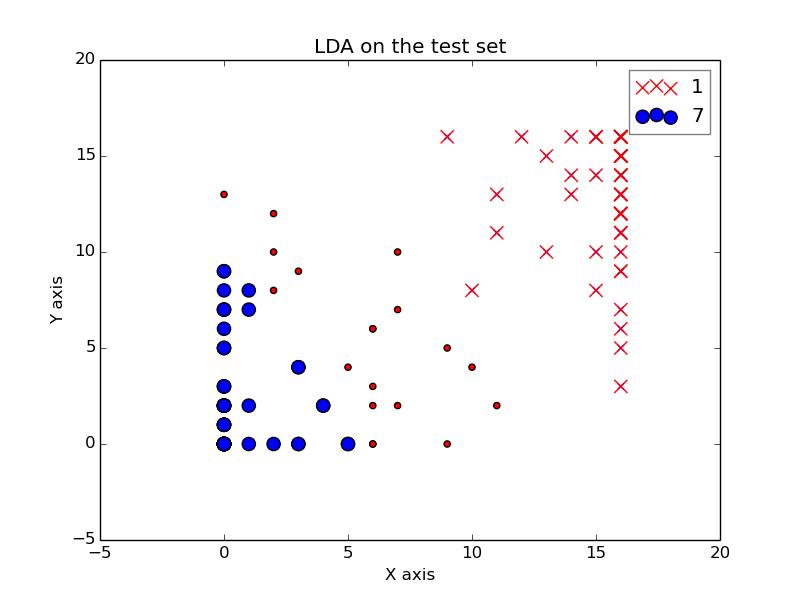
\includegraphics[width=\textwidth]{../LDAtestset.png}
                \caption{Test set}
        \end{subfigure}
        \caption{Results of LDA Prediction}
        \label{img6}
\end{figure}


\FloatBarrier


\section{Complete Code}

\lstinputlisting[language=Python]{../ex02.py}

\end{document}
%------------------------------------------------------------------------------%                                    
